% ****************************************************************************************
% *****************          EJERCICIO DE ALGORITMOS           ***************************
% ****************************************************************************************


% =======================================================
% =======         HEADER FOR DOCUMENT        ============
% =======================================================
    
    % *********   HEADERS AND FOOTERS ********
    \def\ProjectAuthorLink{https://github.com/SoyOscarRH}           %Just to keep it in line
    \def\ProjectNameLink{\ProjectAuthorLink/Proyect}                %Link to Proyect

    % *********   DOCUMENT ITSELF   **************
    \documentclass[12pt, fleqn]{article}                            %Type of document and size of font
    \usepackage[spanish]{babel}                                     %Please use spanish
    \usepackage[utf8]{inputenc}                                     %Please use spanish - UFT
    \usepackage[margin = 1.2in]{geometry}                           %Margins and Geometry pacakge
    \usepackage{ifthen}                                             %Allow simple programming
    \usepackage{hyperref}                                           %Create MetaData for a PDF and LINKS!
    \usepackage{pdfpages}                                           %Create MetaData for a PDF and LINKS!
    \hypersetup{pageanchor = false}                                 %Solve 'double page 1' warnings in build
    \setlength{\parindent}{0pt}                                     %Eliminate ugly indentation
    \author{Oscar Andrés Rosas}                                     %Who I am

    % *********   LANGUAJE    *****************
    \usepackage[T1]{fontenc}                                        %Please use spanish
    \usepackage{textcmds}                                           %Allow us to use quoutes
    \usepackage{changepage}                                         %Allow us to use identate paragraphs
    \usepackage{anyfontsize}                                        %All the sizes

    % *********   MATH AND HIS STYLE  *********
    \usepackage{ntheorem, amsmath, amssymb, amsfonts}               %All fucking math, I want all!
    \usepackage{mathrsfs, mathtools, empheq}                        %All fucking math, I want all!
    \usepackage{cancel}                                             %Negate symbol
    \usepackage{centernot}                                          %Allow me to negate a symbol
    \decimalpoint                                                   %Use decimal point

    % *********   GRAPHICS AND IMAGES *********
    \usepackage{graphicx}                                           %Allow to create graphics
    \usepackage{float}                                              %For images
    \usepackage{wrapfig}                                            %Allow to create images
    \graphicspath{ {Graphics/} }                                    %Where are the images :D

    % *********   LISTS AND TABLES ***********
    \usepackage{listings, listingsutf8}                             %We will be using code here
    \usepackage[inline]{enumitem}                                   %We will need to enumarate
    \usepackage{tasks}                                              %Horizontal lists
    \usepackage{longtable}                                          %Lets make tables awesome
    \usepackage{booktabs}                                           %Lets make tables awesome
    \usepackage{tabularx}                                           %Lets make tables awesome
    \usepackage{multirow}                                           %Lets make tables awesome
    \usepackage{multicol}                                           %Create multicolumns

    % *********   HEADERS AND FOOTERS ********
    \usepackage{fancyhdr}                                           %Lets make awesome headers/footers
    \pagestyle{fancy}                                               %Lets make awesome headers/footers
    \setlength{\headheight}{16pt}                                   %Top line
    \setlength{\parskip}{0.5em}                                     %Top line
    \renewcommand{\footrulewidth}{0.5pt}                            %Bottom line

    \lhead {                                                        %Left Header
        \hyperlink{section.\arabic{section}}                        %Make a link to the current chapter
        {\normalsize{\textsc{\nouppercase{\leftmark}}}}             %And fot it put the name
    }

    \rhead {                                                        %Right Header
        \hyperlink{section.\arabic{section}.\arabic{subsection}}    %Make a link to the current chapter
            {\footnotesize{\textsc{\nouppercase{\rightmark}}}}      %And fot it put the name
    }

    \rfoot{\textsc{\small{\hyperref[sec:Index]{Ve al Índice}}}}     %This will always be a footer  

    \fancyfoot[L]{                                                  %Algoritm for a changing footer
        \ifthenelse{\isodd{\value{page}}}                           %IF ODD PAGE:
            {\href{https://compilandoconocimiento.com/nosotros/}    %DO THIS:
                {\footnotesize                                      %Send the page
                    {\textsc{Oscar Andrés Rosas}}}}                 %Send the page
            {\href{https://compilandoconocimiento.com}              %ELSE DO THIS: 
                {\footnotesize                                      %Send the author
                    {\textsc{Arturo Rivas Rojas}}}}            %Send the author
    }
    
    
    
% =======================================================
% ===================   COMMANDS    =====================
% =======================================================

    % =========================================
    % =======   NEW ENVIRONMENTS   ============
    % =========================================
    \newenvironment{Indentation}[1][0.75em]                         %Use: \begin{Inde...}[Num]...\end{Inde...}
        {\begin{adjustwidth}{#1}{}}                                 %If you dont put nothing i will use 0.75 em
        {\end{adjustwidth}}                                         %This indentate a paragraph
    \newenvironment{SmallIndentation}[1][0.75em]                    %Use: The same that we upper one, just 
        {\begin{adjustwidth}{#1}{}\begin{footnotesize}}             %footnotesize size of letter by default
        {\end{footnotesize}\end{adjustwidth}}                       %that's it

    \newenvironment{MultiLineEquation}[1]                           %Use: To create MultiLine equations
        {\begin{equation}\begin{alignedat}{#1}}                     %Use: \begin{Multi..}{Num. de Columnas}
        {\end{alignedat}\end{equation}}                             %And.. that's it!
    \newenvironment{MultiLineEquation*}[1]                          %Use: To create MultiLine equations
        {\begin{equation*}\begin{alignedat}{#1}}                    %Use: \begin{Multi..}{Num. de Columnas}
        {\end{alignedat}\end{equation*}}                            %And.. that's it!
    

    % =========================================
    % == GENERAL TEXT & SYMBOLS ENVIRONMENTS ==
    % =========================================
    
    % =====  TEXT  ======================
    \newcommand \Quote {\qq}                                        %Use: \Quote to use quotes
    \newcommand \Over {\overline}                                   %Use: \Bar to use just for short
    \newcommand \ForceNewLine {$\Space$\\}                          %Use it in theorems for example

    % =====  SPACES  ====================
    \DeclareMathOperator \Space {\quad}                             %Use: \Space for a cool mega space
    \DeclareMathOperator \MegaSpace {\quad \quad}                   %Use: \MegaSpace for a cool mega mega space
    \DeclareMathOperator \MiniSpace {\;}                            %Use: \Space for a cool mini space
    
    % =====  MATH TEXT  =================
    \newcommand \Such {\MiniSpace | \MiniSpace}                     %Use: \Such like in sets
    \newcommand \Also {\MiniSpace \text{y} \MiniSpace}              %Use: \Also so it's look cool
    \newcommand \Remember[1]{\Space\text{\scriptsize{#1}}}          %Use: \Remember so it's look cool
    
    % =====  THEOREMS  ==================
    \newtheorem{Theorem}{Teorema}[section]                          %Use: \begin{Theorem}[Name]\label{Nombre}...
    \newtheorem{Corollary}{Colorario}[Theorem]                      %Use: \begin{Corollary}[Name]\label{Nombre}...
    \newtheorem{Lemma}[Theorem]{Lemma}                              %Use: \begin{Lemma}[Name]\label{Nombre}...
    \newtheorem{Definition}{Definición}[section]                    %Use: \begin{Definition}[Name]\label{Nombre}...
    \theoremstyle{break}                                            %THEOREMS START 1 SPACE AFTER

    % =====  LOGIC  =====================
    \newcommand \lIff    {\leftrightarrow}                          %Use: \lIff for logic iff
    \newcommand \lEqual  {\MiniSpace \Leftrightarrow \MiniSpace}    %Use: \lEqual for a logic double arrow
    \newcommand \lInfire {\MiniSpace \Rightarrow \MiniSpace}        %Use: \lInfire for a logic infire
    \newcommand \lLongTo {\longrightarrow}                          %Use: \lLongTo for a long arrow

    % =====  FAMOUS SETS  ===============
    \DeclareMathOperator \Naturals     {\mathbb{N}}                 %Use: \Naturals por Notation
    \DeclareMathOperator \Primes       {\mathbb{P}}                 %Use: \Primes por Notation
    \DeclareMathOperator \Integers     {\mathbb{Z}}                 %Use: \Integers por Notation
    \DeclareMathOperator \Racionals    {\mathbb{Q}}                 %Use: \Racionals por Notation
    \DeclareMathOperator \Reals        {\mathbb{R}}                 %Use: \Reals por Notation
    \DeclareMathOperator \Complexs     {\mathbb{C}}                 %Use: \Complex por Notation
    \DeclareMathOperator \GenericField {\mathbb{F}}                 %Use: \GenericField por Notation
    \DeclareMathOperator \VectorSet    {\mathbb{V}}                 %Use: \VectorSet por Notation
    \DeclareMathOperator \SubVectorSet {\mathbb{W}}                 %Use: \SubVectorSet por Notation
    \DeclareMathOperator \Polynomials  {\mathbb{P}}                 %Use: \Polynomials por Notation
    \DeclareMathOperator \VectorSpace  {\VectorSet_{\GenericField}} %Use: \VectorSpace por Notation
    \DeclareMathOperator \LinealTransformation {\mathcal{T}}        %Use: \LinealTransformation for a cool T
    \DeclareMathOperator \LinTrans {\mathcal{T}}                    %Use: \LinTrans for a cool T


    % =====  CONTAINERS   ===============
    \newcommand{\Set}[1]    {\left\{ \; #1 \; \right\}}             %Use: \Set {Info} for INTELLIGENT space 
    \newcommand{\bigSet}[1] {\big\{  \; #1 \; \big\}}               %Use: \bigSet  {Info} for space 
    \newcommand{\BigSet}[1] {\Big\{  \; #1 \; \Big\}}               %Use: \BigSet  {Info} for space 
    \newcommand{\biggSet}[1]{\bigg\{ \; #1 \; \bigg\}}              %Use: \biggSet {Info} for space 
    \newcommand{\BiggSet}[1]{\Bigg\{ \; #1 \; \Bigg\}}              %Use: \BiggSet {Info} for space 
    
    \newcommand{\Brackets}[1]    {\left[ #1 \right]}                %Use: \Brackets {Info} for INTELLIGENT space
    \newcommand{\bigBrackets}[1] {\big[ \; #1 \; \big]}             %Use: \bigBrackets  {Info} for space 
    \newcommand{\BigBrackets}[1] {\Big[ \; #1 \; \Big]}             %Use: \BigBrackets  {Info} for space 
    \newcommand{\biggBrackets}[1]{\bigg[ \; #1 \; \bigg]}           %Use: \biggBrackets {Info} for space 
    \newcommand{\BiggBrackets}[1]{\Bigg[ \; #1 \; \Bigg]}           %Use: \BiggBrackets {Info} for space 
    
    \newcommand{\Wrap}[1]    {\left( #1 \right)}                    %Use: \Wrap {Info} for INTELLIGENT space
    \newcommand{\bigWrap}[1] {\big( \; #1 \; \big)}                 %Use: \bigBrackets  {Info} for space 
    \newcommand{\BigWrap}[1] {\Big( \; #1 \; \Big)}                 %Use: \BigBrackets  {Info} for space 
    \newcommand{\biggWrap}[1]{\bigg( \; #1 \; \bigg)}               %Use: \biggBrackets {Info} for space 
    \newcommand{\BiggWrap}[1]{\Bigg( \; #1 \; \Bigg)}               %Use: \BiggBrackets {Info} for space 
    
    \newcommand{\Generate}[1]{\left\langle #1 \right\rangle}        %Use: \Generate {Info} <>
    \newcommand{\Floor}[1]{\left \lfloor #1 \right \rfloor}         %Use: \Floor {Info} for floor 
    \newcommand{\Ceil}[1]{\left \lceil #1 \right \rceil }           %Use: \Ceil {Info} for ceil

    % =====  BETTERS MATH COMMANDS   =====
    \newcommand{\pfrac}[2]{\Wrap{\dfrac{#1}{#2}}}                   %Use: Put fractions in parentesis

    % =========================================
    % ====   LINEAL ALGEBRA & VECTORS    ======
    % =========================================

    % ===== UNIT VECTORS  ================
    \newcommand{\hati} {\hat{\imath}}                               %Use: \hati for unit vector    
    \newcommand{\hatj} {\hat{\jmath}}                               %Use: \hatj for unit vector    
    \newcommand{\hatk} {\hat{k}}                                    %Use: \hatk for unit vector

    % ===== FN LINEAL TRANSFORMATION  ====
    \newcommand{\FnLinTrans}[1]{\mathcal{T}\Wrap{#1}}               %Use: \FnLinTrans for a cool T
    \newcommand{\VecLinTrans}[1]{\mathcal{T}\pVector{#1}}           %Use: \LinTrans for a cool T
    \newcommand{\FnLinealTransformation}[1]{\mathcal{T}\Wrap{#1}}   %Use: \FnLinealTransformation

    % ===== MAGNITUDE  ===================
    \newcommand{\abs}[1]{\left\lvert #1 \right\lvert}               %Use: \abs{expression} for |x|
    \newcommand{\Abs}[1]{\left\lVert #1 \right\lVert}               %Use: \Abs{expression} for ||x||
    \newcommand{\Mag}[1]{\left| #1 \right|}                         %Use: \Mag {Info} 
    
    \newcommand{\bVec}[1]{\mathbf{#1}}                              %Use for bold type of vector
    \newcommand{\lVec}[1]{\overrightarrow{#1}}                      %Use for a long arrow over a vector
    \newcommand{\uVec}[1]{\mathbf{\hat{#1}}}                        %Use: Unitary Vector Example: $\uVec{i}

    % ===== ALL FOR DOT PRODUCT  =========
    \makeatletter                                                   %WTF! IS THIS
    \newcommand*\dotP{\mathpalette\dotP@{.5}}                       %Use: \dotP for dot product
    \newcommand*\dotP@[2] {\mathbin {                               %WTF! IS THIS            
        \vcenter{\hbox{\scalebox{#2}{$\m@th#1\bullet$}}}}           %WTF! IS THIS
    }                                                               %WTF! IS THIS
    \makeatother                                                    %WTF! IS THIS

    % === WRAPPERS FOR COLUMN VECTOR ===
    \newcommand{\pVector}[1]                                        %Use: \pVector {Matrix Notation} use parentesis
        { \ensuremath{\begin{pmatrix}#1\end{pmatrix}} }             %Example: \pVector{a\\b\\c} or \pVector{a&b&c} 
    \newcommand{\lVector}[1]                                        %Use: \lVector {Matrix Notation} use a abs 
        { \ensuremath{\begin{vmatrix}#1\end{vmatrix}} }             %Example: \lVector{a\\b\\c} or \lVector{a&b&c} 
    \newcommand{\bVector}[1]                                        %Use: \bVector {Matrix Notation} use a brackets 
        { \ensuremath{\begin{bmatrix}#1\end{bmatrix}} }             %Example: \bVector{a\\b\\c} or \bVector{a&b&c} 
    \newcommand{\Vector}[1]                                         %Use: \Vector {Matrix Notation} no parentesis
        { \ensuremath{\begin{matrix}#1\end{matrix}} }               %Example: \Vector{a\\b\\c} or \Vector{a&b&c}

    % === MAKE MATRIX BETTER  =========
    \makeatletter                                                   %Example: \begin{matrix}[cc|c]
    \renewcommand*\env@matrix[1][*\c@MaxMatrixCols c] {             %WTF! IS THIS
        \hskip -\arraycolsep                                        %WTF! IS THIS
        \let\@ifnextchar\new@ifnextchar                             %WTF! IS THIS
        \array{#1}                                                  %WTF! IS THIS
    }                                                               %WTF! IS THIS
    \makeatother                                                    %WTF! IS THIS

    % =========================================
    % =======   FAMOUS FUNCTIONS   ============
    % =========================================

    % == TRIGONOMETRIC FUNCTIONS  ====
    \newcommand{\Cos}[1] {\cos\Wrap{#1}}                            %Simple wrappers
    \newcommand{\Sin}[1] {\sin\Wrap{#1}}                            %Simple wrappers
    \newcommand{\Tan}[1] {tan\Wrap{#1}}                             %Simple wrappers
    
    \newcommand{\Sec}[1] {sec\Wrap{#1}}                             %Simple wrappers
    \newcommand{\Csc}[1] {csc\Wrap{#1}}                             %Simple wrappers
    \newcommand{\Cot}[1] {cot\Wrap{#1}}                             %Simple wrappers

    % === COMPLEX ANALYSIS TRIG ======
    \newcommand \Cis[1]  {\Cos{#1} + i \Sin{#1}}                    %Use: \Cis for cos(x) + i sin(x)
    \newcommand \pCis[1] {\Wrap{\Cis{#1}}}                          %Use: \pCis for the same with parantesis
    \newcommand \bCis[1] {\Brackets{\Cis{#1}}}                      %Use: \bCis for the same with Brackets


    % =========================================
    % ===========     CALCULUS     ============
    % =========================================

    % ====== TRANSFORMS =============
    \newcommand{\FourierT}[1]{\mathscr{F} \left\{ #1 \right\} }     %Use: \FourierT {Funtion}
    \newcommand{\InvFourierT}[1]{\mathscr{F}^{-1}\left\{#1\right\}} %Use: \InvFourierT {Funtion}

    % ====== DERIVATIVES ============
    \newcommand \MiniDerivate[1][x] {\dfrac{d}{d #1}}               %Use: \MiniDerivate[var] for simple use [var]
    \newcommand \Derivate[2] {\dfrac{d \; #1}{d #2}}                %Use: \Derivate [f(x)][x]
    \newcommand \MiniUpperDerivate[2] {\dfrac{d^{#2}}{d#1^{#2}}}    %Mini Derivate High Orden Derivate -- [x][pow]
    \newcommand \UpperDerivate[3] {\dfrac{d^{#3} \; #1}{d#2^{#3}}}  %Complete High Orden Derivate -- [f(x)][x][pow]
    
    \newcommand \MiniPartial[1][x] {\dfrac{\partial}{\partial #1}}  %Use: \MiniDerivate for simple use [var]
    \newcommand \Partial[2] {\dfrac{\partial \; #1}{\partial #2}}   %Complete Partial Derivate -- [f(x)][x]
    \newcommand \MiniUpperPartial[2]                                %Mini Derivate High Orden Derivate -- [x][pow] 
        {\dfrac{\partial^{#2}}{\partial #1^{#2}}}                   %Mini Derivate High Orden Derivate
    \newcommand \UpperPartial[3]                                    %Complete High Orden Derivate -- [f(x)][x][pow]
        {\dfrac{\partial^{#3} \; #1}{\partial#2^{#3}}}              %Use: \UpperDerivate for simple use

    \DeclareMathOperator \Evaluate  {\Big|}                         %Use: \Evaluate por Notation

    % =========================================
    % ========    GENERAL STYLE     ===========
    % =========================================
    
    % =====  COLORS ==================
    \definecolor{RedMD}{HTML}{F44336}                               %Use: Color :D        
    \definecolor{Red100MD}{HTML}{FFCDD2}                            %Use: Color :D        
    \definecolor{Red200MD}{HTML}{EF9A9A}                            %Use: Color :D        
    \definecolor{Red300MD}{HTML}{E57373}                            %Use: Color :D        
    \definecolor{Red700MD}{HTML}{D32F2F}                            %Use: Color :D 

    \definecolor{PurpleMD}{HTML}{9C27B0}                            %Use: Color :D        
    \definecolor{Purple100MD}{HTML}{E1BEE7}                         %Use: Color :D        
    \definecolor{Purple200MD}{HTML}{EF9A9A}                         %Use: Color :D        
    \definecolor{Purple300MD}{HTML}{BA68C8}                         %Use: Color :D        
    \definecolor{Purple700MD}{HTML}{7B1FA2}                         %Use: Color :D 

    \definecolor{IndigoMD}{HTML}{3F51B5}                            %Use: Color :D        
    \definecolor{Indigo100MD}{HTML}{C5CAE9}                         %Use: Color :D        
    \definecolor{Indigo200MD}{HTML}{9FA8DA}                         %Use: Color :D        
    \definecolor{Indigo300MD}{HTML}{7986CB}                         %Use: Color :D        
    \definecolor{Indigo700MD}{HTML}{303F9F}                         %Use: Color :D 

    \definecolor{BlueMD}{HTML}{2196F3}                              %Use: Color :D        
    \definecolor{Blue100MD}{HTML}{BBDEFB}                           %Use: Color :D        
    \definecolor{Blue200MD}{HTML}{90CAF9}                           %Use: Color :D        
    \definecolor{Blue300MD}{HTML}{64B5F6}                           %Use: Color :D        
    \definecolor{Blue700MD}{HTML}{1976D2}                           %Use: Color :D        
    \definecolor{Blue900MD}{HTML}{0D47A1}                           %Use: Color :D  

    \definecolor{CyanMD}{HTML}{00BCD4}                              %Use: Color :D        
    \definecolor{Cyan100MD}{HTML}{B2EBF2}                           %Use: Color :D        
    \definecolor{Cyan200MD}{HTML}{80DEEA}                           %Use: Color :D        
    \definecolor{Cyan300MD}{HTML}{4DD0E1}                           %Use: Color :D        
    \definecolor{Cyan700MD}{HTML}{0097A7}                           %Use: Color :D        
    \definecolor{Cyan900MD}{HTML}{006064}                           %Use: Color :D 

    \definecolor{TealMD}{HTML}{009688}                              %Use: Color :D        
    \definecolor{Teal100MD}{HTML}{B2DFDB}                           %Use: Color :D        
    \definecolor{Teal200MD}{HTML}{80CBC4}                           %Use: Color :D        
    \definecolor{Teal300MD}{HTML}{4DB6AC}                           %Use: Color :D        
    \definecolor{Teal700MD}{HTML}{00796B}                           %Use: Color :D        
    \definecolor{Teal900MD}{HTML}{004D40}                           %Use: Color :D 

    \definecolor{GreenMD}{HTML}{4CAF50}                             %Use: Color :D        
    \definecolor{Green100MD}{HTML}{C8E6C9}                          %Use: Color :D        
    \definecolor{Green200MD}{HTML}{A5D6A7}                          %Use: Color :D        
    \definecolor{Green300MD}{HTML}{81C784}                          %Use: Color :D        
    \definecolor{Green700MD}{HTML}{388E3C}                          %Use: Color :D        
    \definecolor{Green900MD}{HTML}{1B5E20}                          %Use: Color :D

    \definecolor{AmberMD}{HTML}{FFC107}                             %Use: Color :D        
    \definecolor{Amber100MD}{HTML}{FFECB3}                          %Use: Color :D        
    \definecolor{Amber200MD}{HTML}{FFE082}                          %Use: Color :D        
    \definecolor{Amber300MD}{HTML}{FFD54F}                          %Use: Color :D        
    \definecolor{Amber700MD}{HTML}{FFA000}                          %Use: Color :D        
    \definecolor{Amber900MD}{HTML}{FF6F00}                          %Use: Color :D

    \definecolor{BlueGreyMD}{HTML}{607D8B}                          %Use: Color :D        
    \definecolor{BlueGrey100MD}{HTML}{CFD8DC}                       %Use: Color :D        
    \definecolor{BlueGrey200MD}{HTML}{B0BEC5}                       %Use: Color :D        
    \definecolor{BlueGrey300MD}{HTML}{90A4AE}                       %Use: Color :D        
    \definecolor{BlueGrey700MD}{HTML}{455A64}                       %Use: Color :D        
    \definecolor{BlueGrey900MD}{HTML}{263238}                       %Use: Color :D        

    \definecolor{DeepPurpleMD}{HTML}{673AB7}                        %Use: Color :D

    \newcommand{\Color}[2]{\textcolor{#1}{#2}}                      %Simple color environment
    \newenvironment{ColorText}[1]                                   %Use: \begin{ColorText}
        { \leavevmode\color{#1}\ignorespaces }                      %That's is!

    % =====  CODE EDITOR =============
    \lstdefinestyle{CompilandoStyle} {                              %This is Code Style
        backgroundcolor     = \color{BlueGrey900MD},                %Background Color  
        basicstyle          = \tiny\color{white},                   %Style of text
        commentstyle        = \color{BlueGrey200MD},                %Comment style
        stringstyle         = \color{Green300MD},                   %String style
        keywordstyle        = \color{Blue300MD},                    %keywords style
        numberstyle         = \tiny\color{TealMD},                  %Size of a number
        frame               = shadowbox,                            %Adds a frame around the code
        breakatwhitespace   = true,                                 %Style   
        breaklines          = true,                                 %Style   
        showstringspaces    = false,                                %Hate those spaces                  
        breaklines          = true,                                 %Style                   
        keepspaces          = true,                                 %Style                   
        numbers             = left,                                 %Style                   
        numbersep           = 10pt,                                 %Style 
        xleftmargin         = \parindent,                           %Style 
        tabsize             = 4,                                    %Style
        inputencoding       = utf8/latin1                           %Allow me to use special chars
    }
 
    \lstset{style = CompilandoStyle}                                %Use this style


% =====================================================
% ============        COVER PAGE       ================
% =====================================================
\begin{document}
\begin{titlepage}
    
    % ============ TITLE PAGE STYLE  ================
    \definecolor{TitlePageColor}{cmyk}{1,.60,0,.40}                 %Simple colors
    \definecolor{ColorSubtext}{cmyk}{1,.50,0,.10}                   %Simple colors
    \newgeometry{left=0.25\textwidth}                               %Defines an Offset
    \pagecolor{TitlePageColor}                                      %Make it this Color to page
    \color{white}                                                   %General things should be white

    % ===== MAKE SOME SPACE =========
    \vspace                                                         %Give some space
    \baselineskip                                                   %But we need this to up command

    % ============ NAME OF THE PROJECT  ============
    \makebox[0pt][l]{\rule{1.3\textwidth}{3pt}}                     %Make a cool line
    
    \href{https://compilandoconocimiento.com/}                      %Link to project
    {\textbf{\textsc{\Huge ESCOM - IPN}}}\\[2.7cm]                  %Name of project   

    % ============ NAME OF THE BOOK  ===============
    \href{https://github.com/CompilandoConocimiento/}               %Link to Author
    {\fontsize{65}{78}\selectfont \textbf{Practica 2: }}\\[0.5cm]     %Name of the book
    
    \Huge{Implementación de Checksum para el Encabezado IP, TCP y UDP}

    \textcolor{ColorSubtext}{\textsc{\Huge Redes de Cómputadoras 2CM10}}\\[2cm]%Name of the general theme
    
    \vfill                                                          %Fill the space

    % ============ NAME OF THE AUTHOR  =============
    \href{ProjectAuthorLink}                                        %Link to Author
    {\LARGE \textsf{Oscar Andrés Rosas Hernandez}}                  %Author
    {\LARGE \textsf{Arturo Rivas Rojas}}                            %Author

    % ===== MAKE SOME SPACE =========
    \vspace                                                         %Give some space
    \baselineskip                                                   %But we need this to up command
    
    {\large \textsf{Junio 2018}}                                    %Date

\end{titlepage}


% =====================================================
% ==========      RESTORE TO DOCUMENT      ============
% =====================================================
\restoregeometry                                                    %Restores the geometry
\nopagecolor                                                        %Use to restore the color to white


% =====================================================
% ========                INDICE              =========
% =====================================================
\tableofcontents{}
\label{sec:Index}

\clearpage

    

    % ===============================================================================
    % ============            PROTOCOLO OSI                   =======================
    % ===============================================================================
    \section{Protocolo OSI}


        % ==============================================================
        % =================       DEFINICION          ==================
        % ==============================================================
        \subsection{Definición}

            Antes que nada, es un modelo de referencia. Pretende que los sistemas que son diseñados
            con base en el, se pueden comunicar sin problemas.

        % ==============================================================
        % =================       PARTES              ==================
        % ==============================================================
        \subsection{Partes}

            \begin{itemize}
                
                \item \textbf{Capa Física:} 

                    Se encarga de la transmición de datos, de cadenas de bits no estrucurados sobre
                    el medio físico y esta relacionado con:
                    \begin{itemize}
                        \item Voltaje necasario para representar cada bit
                        \item Cuanto dura cada símbolo, es decir el tiempo de trama
                        \item Si se realiza simultáneamente en ambos sentidos o no
                        \item Como se establece una transmición y como interrumpirla
                        \item Especificar como serán los pines del conector de red, para que sirve
                            cada pin pues
                    \end{itemize}

                \item \textbf{Capa de Enlace de Red:} 

                    Trabaja con direcciónes físicas.

                    Proporciona el servicio de transferencia de datos (tramas) llevando a cabo
                    la sincronización y correción de datos, así como el control de flujo.

                \item \textbf{Capa de Red:}

                    Trabaja con IP (es decir, direcciones lógicas) para poder conectar dos redes. 
                    Es responsable del establecimiento, mantenimiento y cierre de conexión.

                    También brinda las funciones de direccionamiento lógico y enrutamiento.

                    Se direccionan de manera lógica y no física para evitar problemas con el hardware.

                \item \textbf{Capa de Transporte:}

                    Hablaremos de si será un archivo orientado a conexión (TCP), o si no esta orientado
                    a conexión (UDP), es decir la importancia que le damos a si queremos los datos integros
                    o si requerimos gran velocidad.

                    Proporciona seguridad, transferencia y transporte de datos entre los puntos finales
                    también proporcionan mecanismos de control de flujo y de errores en el origen y destino.

                    Esta proporciona el control de la comunicación entre diferentes aplicaciones, establece,
                    gestiona y cierra la comunicación entre aplicaciones

                \clearpage

                \item \textbf{Capa  de Sesión:}

                    Hablaremos los números de puerto, un identificador de programa que nos permite ejecutar
                    varias aplicaciones al mismo tiempo, estas son permite ejecutar unos 65,536 aplicaciones
                    en red TCP y otros 65,536 en UDP. Si, un montón.

                \item \textbf{Presentación:}

                    Poder transmitir los datos de manera transparte y sin importar la arquitectura de las
                    computadoras de origen y destino.

                \item \textbf{Aplicación:}

                    Es donde trabajamos a nivel usario y ... poquito más.

                    Proporciona un medio a los programas de aplicación para acceder a los servicios de red,
                    contiene funciones de administración de aplicaciones distribuidas.

            \end{itemize}


        % ==============================================================
        % =================       PARTES              ==================
        % ==============================================================
        \subsection{Diagrama OSI (Y su comparación vs IP)}

            \begin{figure}[h]
                \centering
                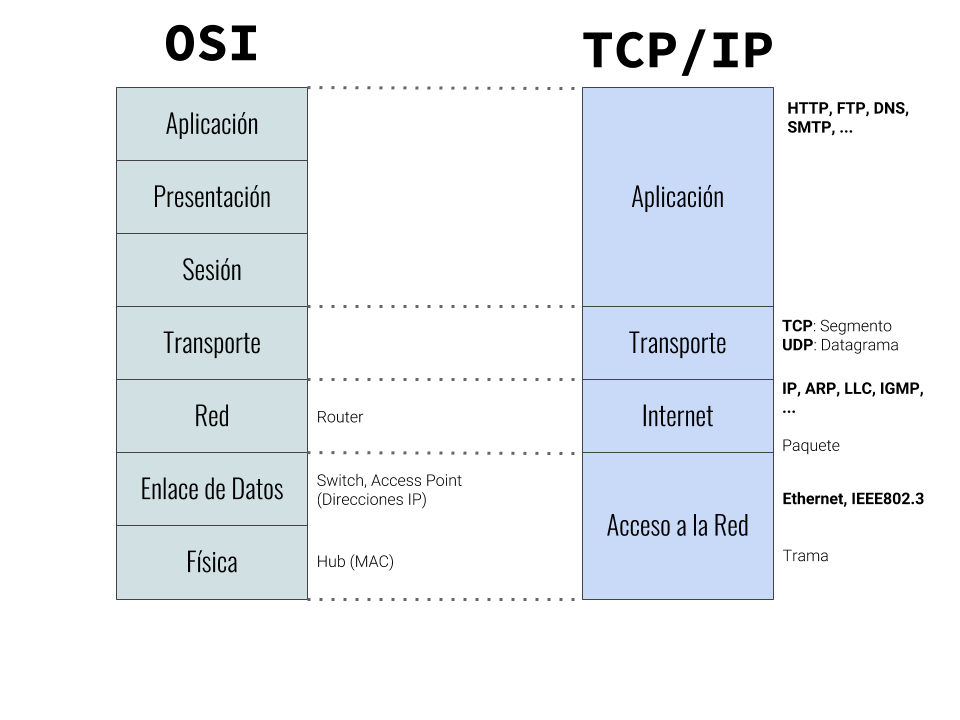
\includegraphics[width=0.9\textwidth]{OSI&IP}
            \end{figure}


    % ===============================================================================
    % ======================      PROTOCOLO IP         ==============================
    % ===============================================================================
    \clearpage
    \section{Protocolo IP}


        % ==============================================================
        % =================       DEFINICIONES        ==================
        % ==============================================================
        \subsection{Definiciones}

            Debido a la cantidad de cables necesarios para conectar cada red con cada otra red del mundo
            no todas las redes tienen una conexión directa, es decir, no existe un cable entre tu red
            lócal y los servidores de Facebook por ejemplo.

            Por eso existe el Protocolo IP que nos permite comunicarnos entre redes.

            En resumén lo que permite es que tu red local solo este conectada a unas pocas redes y a
            varios routers, estos tienen algo llamado una tabla de direcciones, que les permite navegar
            entre redes hasta encontrar su destino. 

            El enrutamiento es parecido a la recursión, en el sentido en que no soluciona tu problema
            sino que solo te lleva un paso más cerca.


            % ==============================================================
            % =================       DIRECCION IP        ==================
            % ==============================================================
            \subsubsection{Direcciones IP}

                Es un identificador único (o casi, ya verás después porque). Necesitamos
                un identificador único porque es lo que nos permite enviar información y que 
                la información que esperamos de regreso sepa a donde llegar.



        % ==============================================================
        % =================     DIRECCION IPv4        ==================
        % ==============================================================
        \clearpage
        \subsection{Dirección IPv4}

            Como fue originalmente desarrollado este esquema podría alocar un identificador
            de \textbf{32 bits} a cada dispositivo que se quisiera conectar a internet.
            Esto nos daría algo así como 4 mill millones de posibles direcciones IP.

            La convención es que estos serían representados como 4 conjuntos de 8 bits representados
            en decimal (una forma un poquito más amigable al público general), es decir:

            \begin{figure}[h]
                \centering
                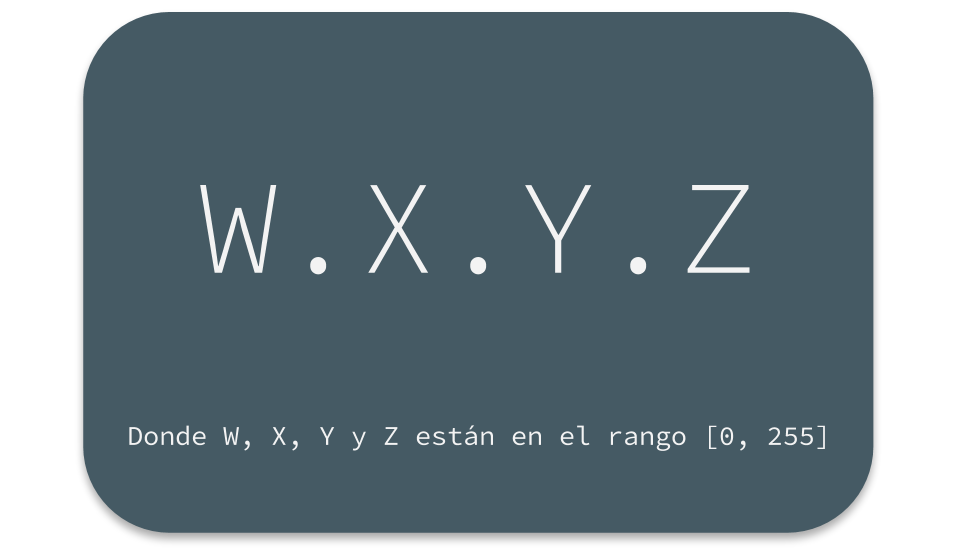
\includegraphics[width=0.80\textwidth]{IPv4}
            \end{figure}

            Por ejemplo una IP v4 válida podría ser $140.247.220.12$. 


            % =========================================================
            % =========   PROBLEMAS CON IP  V4    =====================
            % =========================================================
            \vspace{1.5em}
            \subsubsection{Problemas con IPv4}

                Ahora, recuerda que te dige que IP v4 acepta unos 4 mil millones de direcciones
                válidas, ahora el problema es que ahora mismo hay vivos mas de 7 mil millones
                de personas (A principios del siglo XXI) cada una con seguramente más de un
                dispositivo que quieran conectar a internet.

                Por lo tanto tenemos que encontrar una forma de solucionar esto.



        % ==============================================================
        % =================     DIRECCION IPv6        ==================
        % ==============================================================
        \clearpage
        \subsection{Dirección IPv6}

            Como vimos antes, ahora que parece que la cantidad de direcciones IPv4 se 
            nos esta quedando corta, poco a poco estamos pasando de IPv4 a IPv6 que contará
            con nada menos y nada mas que \textbf{128 bits} para una dirección, es decir
            nos permitirá tener unas más o menos: $340, 282, 366, 920, 938, 463, 463, 374, 607,
            431, 768, 211, 456$ posibles direcciones IP. Un chingo.

            La convención es que estos serían representados como 8 conjuntos de 65535 bits representados
            en hexadecimal (porque de otra manera sale un númerote), es decir:

            \begin{figure}[h]
                \centering
                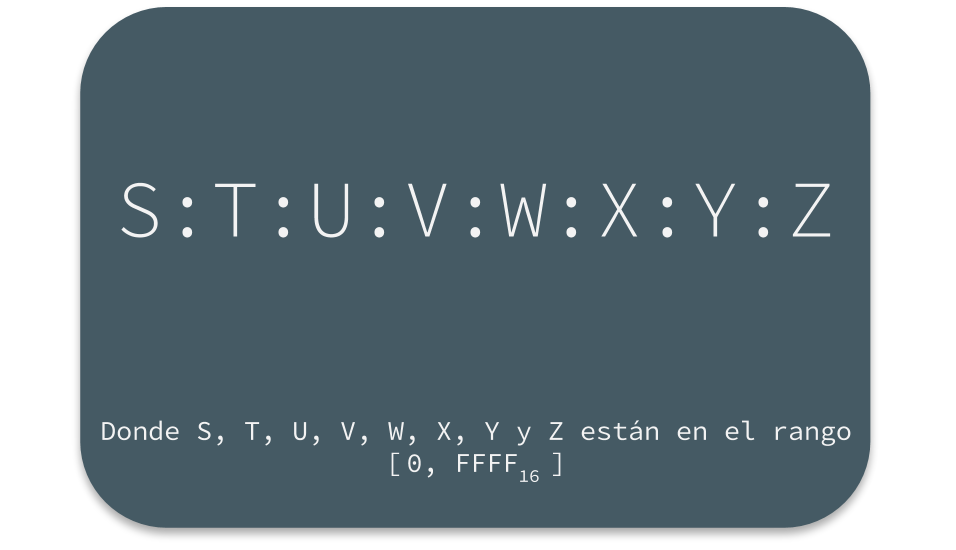
\includegraphics[width=0.80\textwidth]{IPv6}
            \end{figure}

            Por ejemplo una IPv6 podría ser $\Color{BlueGrey700MD}{2001:0DB8:0000:0042:0000:8A2E:0370:7334}$


            % =================================================================
            % ==================   PROBLEMAS CON IPv6      ====================
            % =================================================================
            \clearpage
            \subsection{Haciendo un poco más faciles las Direcciones IPv6}

                Ahora, todo esta mucho mejor que con IPv4, pero tenemos un pequeño
                problema, sus direcciones son moustrosamente enormes, por lo que tuvimos
                que hacer algunas simplificaciones para los humanos:

                \begin{itemize}
                    \item
                        Ignora los ceros dentro de cada grupo de 4 dígitos hexadecimales:

                        % ======== EJEMPLO ========
                        \begin{SmallIndentation}[1em]
                            \textbf{Ejemplo}:
                            \begin{align*}
                                \text{De} \; &\Color{BlueGrey700MD}{2001:0DB8:0000:0042:0000:8A2E:0370:7334}  \\
                                \text{a}  \; &\Color{BlueGrey700MD}{2001:0DB8:0:42:0:8A2E:370:7334} 
                            \end{align*}
                        
                        \end{SmallIndentation}
                        
                    \item 
                        Si tienes un montón de ceros pon $::$ y da por sentado que quien lee esta dirección
                        tiene cerebro y puede entender que ahí van ceros:

                        % ======== EJEMPLO ========
                        \begin{SmallIndentation}[1em]
                            \textbf{Ejemplo}:
                            \begin{align*}
                                \text{De} \; &\Color{BlueGrey700MD}{2001:0DB8:0000:0042:0000:0000:0000:0000}   \\
                                \text{a}  \; &\Color{BlueGrey700MD}{2001:0DB8:0000:0042::}         
                            \end{align*}
                        
                        \end{SmallIndentation}

                \end{itemize}

        % ==============================================================
        % ==========     DIRECCIONES ESPECIALES       ==================
        % ==============================================================
        \clearpage
        \subsection{Direcciones Especiales}

            \begin{itemize}
                \item \textbf{Ausencia de Dirección:} \Color{Blue700MD}{0.0.0.0}
                \item \textbf{Broadcast:} \Color{Blue700MD}{255.255.255.255}
                \item \textbf{Loopback (LocalHost):} \Color{Blue700MD}{127.0.0.0}

                    Esta dirección nunca saldrá de nuestra máquina

                \item \textbf{Direcciones Privadas (RFC 1918):} 

                    Aquí ya se complican las cosas, estas direcciones estan reservadas:
                    \begin{itemize}
                        \item Para la Clase A tenemos el rango \Color{Blue700MD}{10.0.0.0} a \Color{Blue700MD}{10.255.255.255}
                        \item Para la Clase B tenemos el rango \Color{Blue700MD}{172.16.0.0} a \Color{Blue700MD}{172.31.255.255}
                        \item Para la Clase B tenemos el rango \Color{Blue700MD}{192.168.0.0} a \Color{Blue700MD}{192.168.255.255}
                    \end{itemize}

            \end{itemize}



    % ==============================================================================
    % =========================       TCP                 ==========================
    % ==============================================================================
    \clearpage
    \section{Protocolo TCP}



        % ==============================================================
        % =================       HEADER DEL TCP      ==================
        % ==============================================================
        \subsection{Header - Encabezado}

            \begin{figure}[h]
                \centering
                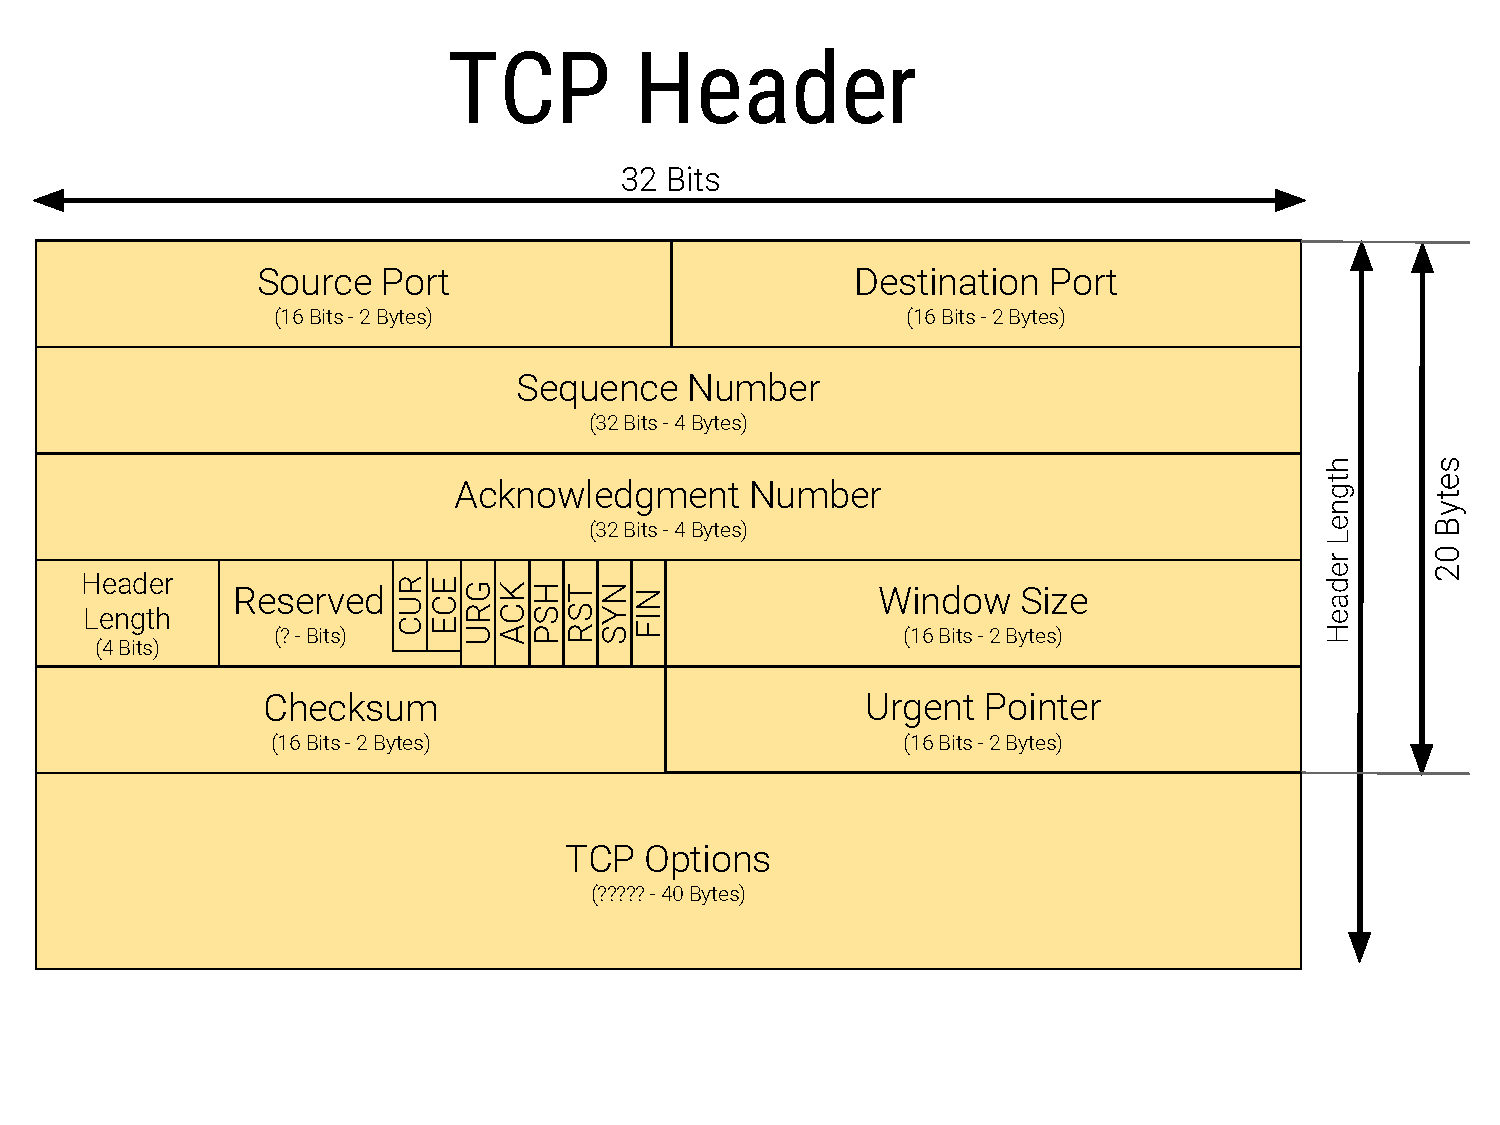
\includegraphics[width=0.95\textwidth]{TCP-Header}
            \end{figure}



    % ==============================================================
    % =================       DEFINICIONES        ==================
    % ==============================================================
    \section{Suma de Comprobación: CheckSum}

        Este algoritmo permite verificar la integridad de la PDU y su calculo es de la siguiente manera:

        \begin{itemize}
            \item Ordena los datos en palabras de 16 bits
            \item Poner ceros en la posición del checksum y sumar con acarreos
            \item Suma cualquier acarreo fuera de los 16 bits
            \item Complementar a uno
        \end{itemize}



    % ===============================================================================
    % =====================           CAPA DE RED      ==============================
    % ===============================================================================
    \section{Capa de Red}

        % ==============================================================
        % =================       DEFINICIONES        ==================
        % ==============================================================
        \vspace{1em}
        \subsection{Definición}

            En esta capa se lleva a cabo el direccionamiento lógico que tiene carácter jerárquico, 
            se selecciona la mejor ruta hacia el destino mediante el uso de tblas de enrutamiento
            a través del uso de protocolos de enrutamiento o por direccionamiento estático.

            Protocolos de Capa de Red son por ejemplo: IP, IPX, RIP, IGRP, Apple Talk.

        % ==============================================================
        % =================       DEFINICIONES        ==================
        % ==============================================================
        \vspace{1em}
        \subsection{Funciones de la capa de red}

            La capa de red define cómo transportar el tráfico de datos entre dispositivos que no 
            están conectados localmente en el mismo dominio de difusíón, es decir, que pertenecen
            a diferentes redes.

            Para conseguir esta comunicación se necesita conocer las direcciones
            lógicas asociadas a cada puesto de origen y de destino y una ruta bien definida a través
            de la red para alcanzar el destino deseado.  La capa de red es independiente de la de
            enlace de datos y, por tanto, puede ser utilizada para conectividad de medios fisicos 
            diferentes.


    % ===============================================================================
    % =====================           CAPA DE TRANSPORTE     ========================
    % ===============================================================================
    \clearpage
    \section{Capa de Transporte}

        % ==============================================================
        % =================       DEFINICIONES        ==================
        % ==============================================================
        \vspace{1em}
        \subsection{Definición}

            Es la encargada de la comunicación confiable entre host, control de flujo y de la corrección
            de errores entre otras cosas. Los datos son divididos en segmentos identificados con un 
            encabezado con un número de puerto que identifica la aplicación de origen. En esta capa
            funcionan protocolos como UDP y TCP, siendo este último uno de los más utilizados debido 
            a su estabilidad y confiabilidad.

        % ==============================================================
        % =================       DEFINICIONES        ==================
        % ==============================================================
        \vspace{1em}
        \subsection{Funciones de la capa de red}

            Para conectar dos dispositivos remotos es necesario establecer una conexión. La capa de
            transporte establece las relgas para esta interconexión. Permite que las estaciones finales
            ensamblen y reensamblen múltiples segmentos del mismo flujo de datos. Esto se hace por medio 
            de identificadores que en TCP/IP reciben el nombre de número de puerto. La capa cuatro permite
            además que las aplicaciones soliciten transporte fiable entre los sistemas. Asegura que los
            segmentos distribuidos serán confirmados al remitente. Coloca de nuevo los segmentos en su
            orden correcto en el receptor. Proporciona control de flujo regulando el tráfico de datos.

            En la capa de transporte, los datos pueden ser transmitidos de forma fiable o no fiable.
            Para IP, el protocolo TCP (Protocolo de control de transporte) es fiable u orientado a 
            conexión con un saludo previo de tres vías, mientras que UDP (Protocolo de datagrama de
            usuario) no es fiable, o no orientado a conexión, donde solo se establece un saludo de dos
            vías antes de enviar los datos.

            TCP utiliza una técnica llamada ventanas, donde se establece la cantidad de envío de paquetes
            antes de transmitir; mientras que en el windowing o de ventana deslizante, el flujo de envío
            de datos es negociado dinámicamente entre el emisor y receptor. En las ventanas deslizantes
            o windowing cada acuse de recibo (ACK) confirma la recepción y el envío siguiente.



    % ==============================================================
    % =====         PROCEO DE ENCAPSULACION DE DATOS       =========
    % ==============================================================
    \clearpage
    \section{Proceso de Encapsulación de Datos}

        El proceso desde que los datos son incorporados al ordenador hasta que se transmiten al medio
        se llama encapsulación. Estos datos son formateados, segmentados, identificados con el 
        direccionamiento lógico y fisico para finalmente ser enviados al medio. A cada capa del modelo
        OSI le corresponde una \textbf{PDU} (Unidad de datos) siguiendo por lo tanto el siguiente orden 
        de encapsulamiento:

        \begin{enumerate}
            \item Datos          
            \item Segmentos      
            \item Paquetes       
            \item Tramas         
            \item Bits           
        \end{enumerate}

        Debido a que posiblemente la cantidad de los datos sea deamasiada, la capa de transporte desde
        el origen se encarga de segmentarlos par así ser empaquetados debidamente, esta misma capa en el 
        destino se encargará de reensamblar los datos y colocarlos en forma secuencial, ya que no siempre
        llegan a su destino en el orden en que han sido segmentados, así mismo acorde al protocolo que se esté
        utilizando habrá o no corrección de errores. Estos segmentos son empaquetados (paquetes o datagramas) e 
        identificados en la capa de red con la dirección lógica o IP correspondiente al origen y destino. 
        Ocurre lo mismo con la dirección MAC en la capa de enlace de datos formándose las tramas o frames para ser
        transmitidos a través de alguna interfaz. Finalmente las tramas son enviadas al medio desde la capa física.
    
        El proceso inverso se realiza en el destino y se llama desencapsulación de datos.



    % ==============================================================================
    % =========================       ETHERNET              ========================
    % ==============================================================================
    \clearpage
    \section{Practica en Si}

        % ==============================================================================
        % =========================       INSTALACION           ========================
        % ==============================================================================
        \subsection{Ideas}

            La práctica consiste en capturar tramas que pasan a través de la tarjeta de red configurada en
            modo promiscuo. A partir de estas tramas analizamos si se trataba de una trama Ethernet, y
            posteriormente si el protocolo de Internet era IP. Para ello utilizamos la librería pcap y
            el código que nos fue proporcionado por el profesor. 

            Para esta práctica supusimos que la trama con la que se trataba era Ethernet, por lo cual no se
            revisó que el campo tipo/longitud fuera mayor o igual a 1500 bytes. 

            Posteriormente, revisamos el byte 13 y 14 de la trama para verificar que el protocolo que se iba
            a utilizar era IPv4, es decir, revisamos que el valor fuera igual a 0x08 en el byte 13 y 0x00en
            el byte 14. 

            Una vez validado el tipo de protocolo como IPv4 continuamos a calcular el checksum para verifica
            posibles errores y dar por buena la trama. 

            El procedimiento que seguimos fue el siguiente: 

            \begin{itemize}
                \item 
                    Calcular la longitud del encabezado IP. 

                \item 
                    Crear un nuevo arreglo de bytes para almacenar el encabezado. 

                \item 
                    Identificar IP de origen e IP destino. 

                \item 
                    Calcular el checksum utilizando el método proporcionado por el profesor. 
            \end{itemize}

            Finalmente, procedimos a identificar el protocolo que se utilizó en la capa de transporte.
            Para esto revisamos el valor del byte 24 de la trama. Si el valor resultaba ser 0x06, sabíamos
            que se trataba de TCP. Por otro lado, si el valor era 0x11, el protocolo era UDP. 

            Para ambos casos se requería calcular el valor del checksum. Sin embargo, para ambos había
            que calcular previamente un pseudo-header que se utiliza en el cálculo del checksum. 

            En cuanto al checksum de TCP, lo calculamos de la manera siguiente:

            \begin{itemize}
                \item 
                    Calculamos la longitud del encabezado TCP. 

                \item 
                    Creamos un nuevo arreglo que almacenaba el encabezado TCP. 

                \item 
                    Creamos un arreglo que iba a contener la información correspondiente al pseudo-header. 

                \item 
                    Agregamos la IP de origen y destino al pseudo-header, en ese orden. 

                \item 
                    Agregamos la información correspondiente a los bytes 9 y 10. En el byte 9 se asigna el valor
                    de 0 y en el byte 10 el valor de 0x06 correspondiente a que se trata de un protocolo TCP. 

                \item 
                    Calculamos la longitud del payload utilizando la longitud total menos la longitud del encabezado
                    IP menos 14 que es la longitud del encabezado TCP. 

                \item 
                    Agregamos la información del payload a los bytes 11 y 12. 

                \item 
                    Creamos un nuevo arreglo que contendrá el payload de TCP y copiamos la información. 

                \item 
                    Creamos un arreglo auxiliar que contendrá: el pseudo-header, el encabezado TCP y el payload. 

                \item 
                    Calculamos el checksum utilizando el arreglo auxiliar. 
            \end{itemize} 

            Por otra parte el checksum de UPD, lo calculamos de la manera siguiente:

            \begin{itemize}
                
                \item 
                    Creamos un arreglo que contendrá el encabezado UDP y copiamos la información. 

                \item 
                    Creamos un arreglo de 12 bytes que nos servirá para crear el pseudo-header. 

                \item 
                    Copiamos el IP origen y el IP destino al pseudo-header. 

                \item 
                    Inicializamos los bytes 9 y 10. El 9 se inicializa a 0x00 y el 10 a 0x11 debido a que
                    se trata del protocolo UDP. 

                \item 
                    Copiamos el encabezado UDP al pseudo-header. 

                \item 
                    Calculamos la longitud del payload: longitud de la trama menos longitud de IP menos longitud de
                    UDP menos 14. 

                \item 
                    Creamos un arreglo de bytes que contendrá el payload y copiamos la información de la trama. 

                \item 
                    Creamos un arreglo temporal de bytes para realizar el cálculo del checksum. Agregamos: pseudo-header,
                    encabezado UDP y el payload, en ese orden. 

                \item 
                    Realizamos el cálculo del checksum. 
             \end{itemize} 



        % ==============================================================================
        % =========================       EVIDENCIAS            ========================
        % ==============================================================================
        \clearpage
        \subsection{Evidencias}

            Primeramente el código:
            \lstinputlisting[language=Java, gobble=12]{Code/Checksum.java}
            \lstinputlisting[language=Java, gobble=12]{Code/Checksumv2.java}

            \clearpage


            Luego ejecutarlo nos dará lo siguiente:
            \begin{figure}[h]
                \centering
                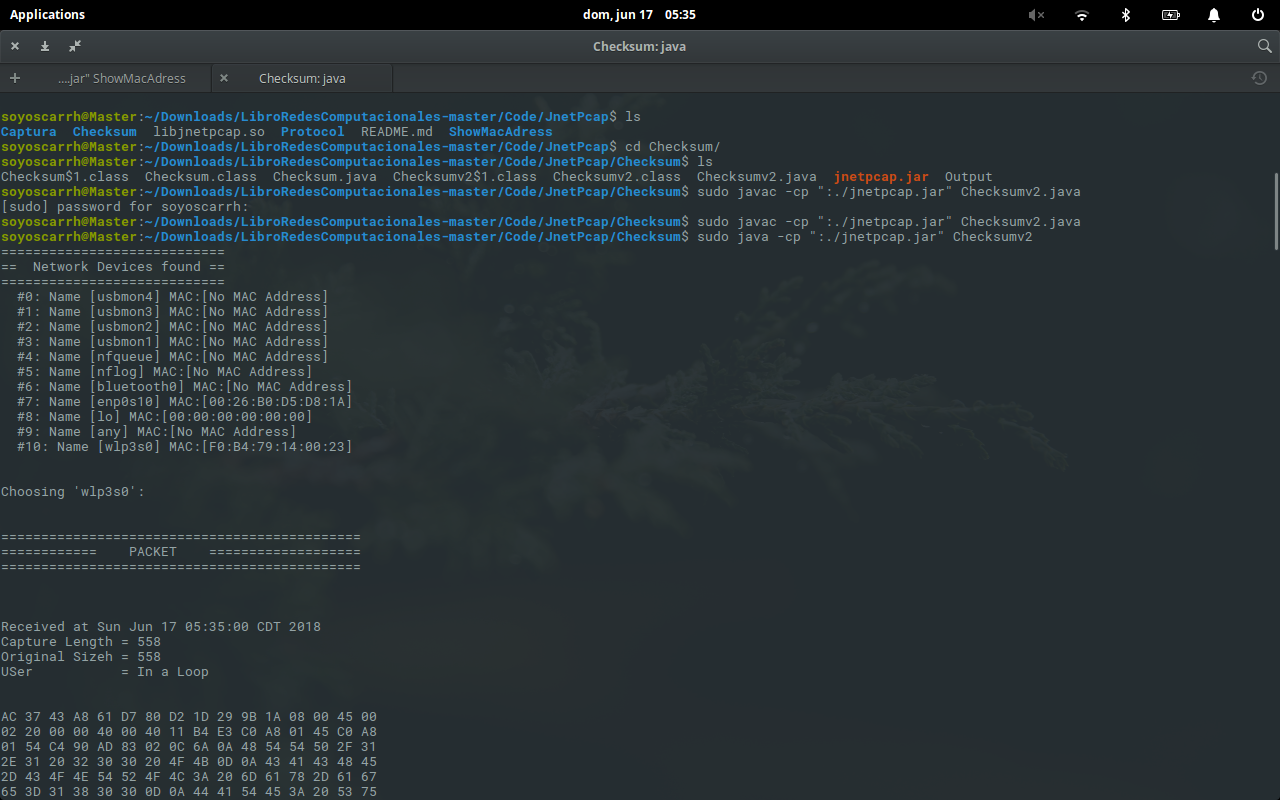
\includegraphics[width=0.85\textwidth]{CheckSum0}
                \caption{Ejemplo}
            \end{figure}

            \begin{figure}[h]
                \centering
                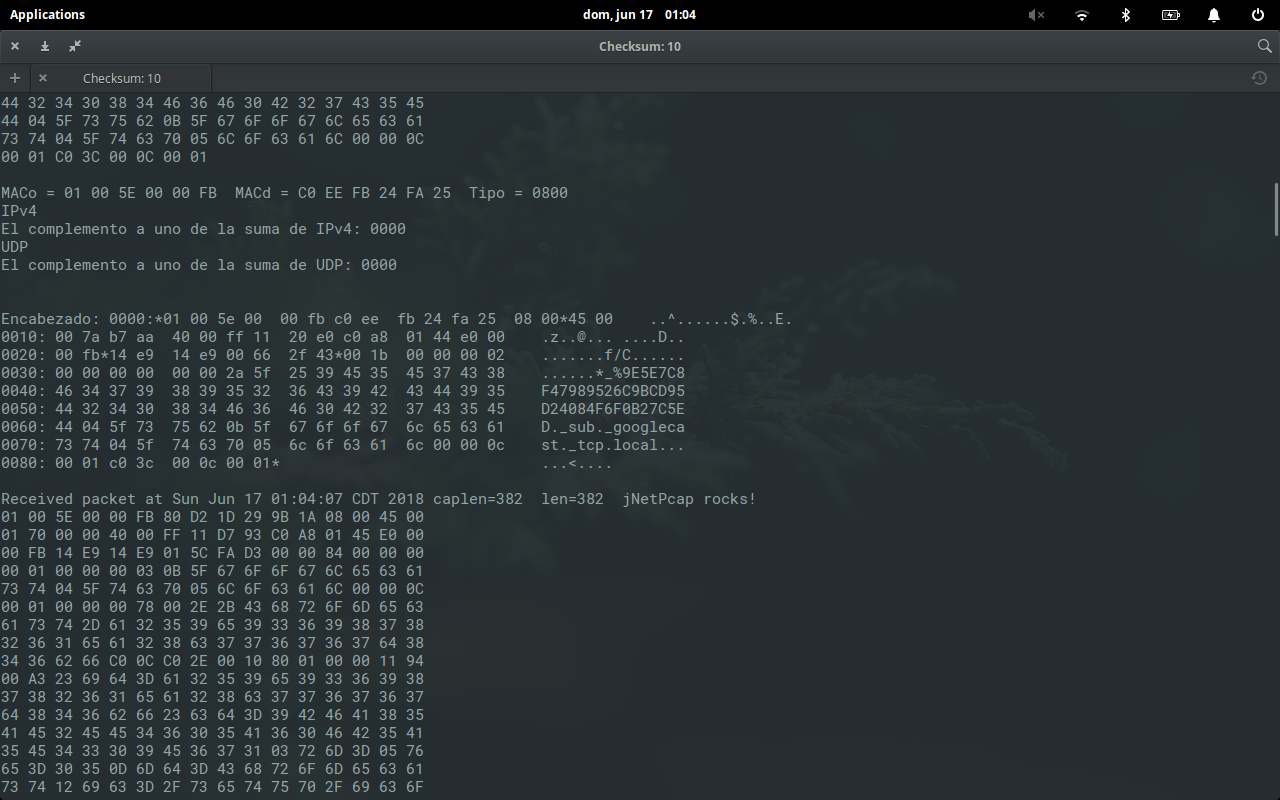
\includegraphics[width=0.85\textwidth]{CheckSum1}
                \caption{Ejemplo}
            \end{figure}

            \begin{figure}[h]
                \centering
                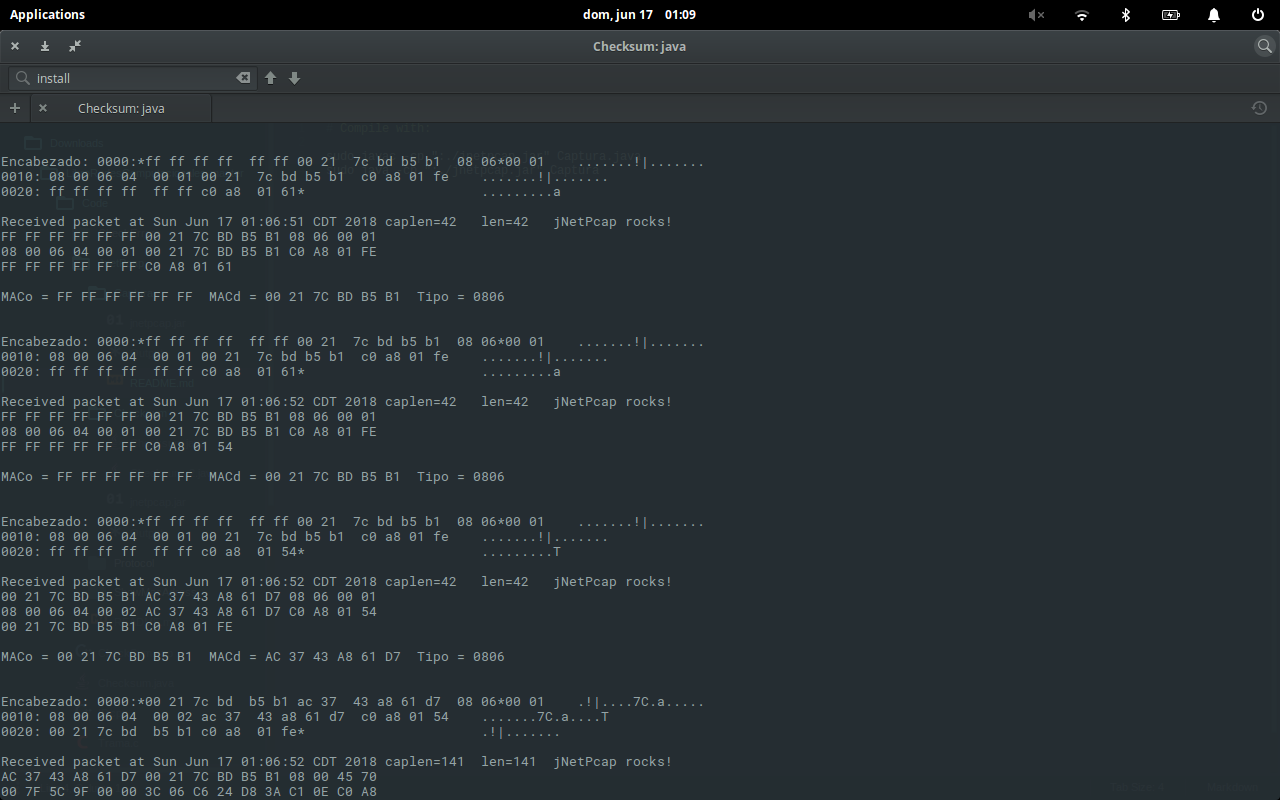
\includegraphics[width=0.85\textwidth]{CheckSum3}
                \caption{Ejemplo}
            \end{figure}

            \begin{figure}[h]
                \centering
                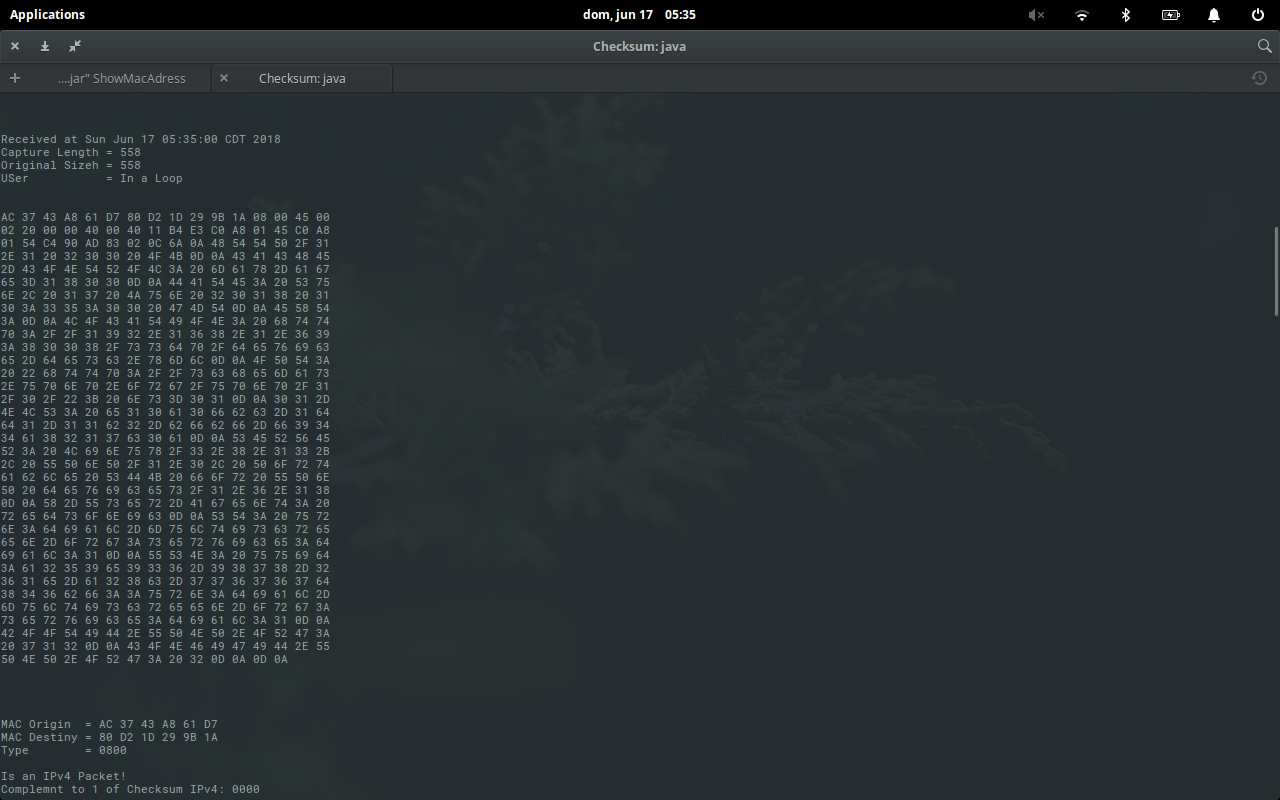
\includegraphics[width=0.85\textwidth]{CheckSum4}
                \caption{Ejemplo}
            \end{figure}


    % ==============================================================================
    % =========================       EVIDENCIAS            ========================
    % ==============================================================================
    \clearpage
    \section{Conclusiones}

        \begin{itemize}
            \item Oscar Andrés Rosas Hernandez

                Al finalizar está práctica pude ver como funciona el algoritmo de Checksum y su
                implementación a un lenguaje de programación
            
                Su funcionamiento ayuda a ver los errores que pueden tener las tramas. También pude ver como
                trabajan las capas de red y de transporte.

                Es esta práctica implementamos el algoritmo de Checksum aplicado a verificar tramas Ethernet.
                Comprobamos que dichas tramas fueran IPv4 verificando que los bytes 13 y 14 sean iguales a 0x0800,
                para posteriormente decidir si el protocolo de la capa de transporte era TCP o UDP. Finalmente,
                comprobamos el campo checksum de estos protocolos. 

                Al correr el programa, verificamos que varias tramas de TCP llegaban incompletas, por lo
                que el checksum era diferente de cero; mientras que las tramas UDP tendían a llegar sin errores
                la mayoría del tiempo. 
            
            \item Arturo Rivas Rojas

                La idea en la que se basa la suma de chequeo de Internet es muy sencilla: se suman todas las
                palabras de 16 bits que conforman el mensaje y se transmite, junto con el mensaje, el resultado
                de dicha suma (este resultado recibe el nombre de checksum). Al llegar el mensaje a su destino,
                el receptor realiza el mismo cálculo sobre los datos recibidos y compara el resultado con el
                checksum recibido. Si cualquiera de los datos transmitidos, incluyendo el mismo checksum, esta
                corrupto, el resultado no concordará y el receptor sabrá que ha ocurrido un error.

                El checksum se realiza de la siguiente manera: los datos que serán procesados (el mensaje) son
                acomodados como una secuencias de enteros de 16 bits. Estos enteros se suman utilizando aritmética
                complemento a uno para 16 bits y, para generar el checksum, se toma el complemento a uno para 16 bits
                del resultado.

                Lo más importante de esta práctica, es la utilización del algoritmo de checksum para identificar
                los errores en una trama, la cual, asumimos inicialmente, que es una trama Ethernet. El checksum
                se validó con base en el protocolo IPv4 y una vez que se ha dado por buena una trama, posteriormente
                verificamos si el protocolo para el transporte es TCP o UDP, en lo que se utilizó el valor calculado
                del checksum, en el que intervenía un pseudo-header. 

            \end{itemize}


    % ===============================================
    % ========        BIBLIO      ===================
    % ===============================================
    \begin{thebibliography}{10}

        \bibitem{CodeName1} 
            E. Ariganello, Redes Cisco. Guıa de estudio para la certificacion CCNA 640-802, 2da Edicion, 201

    \end{thebibliography}


        

\end{document}